\documentclass[12pt,fleqn]{article}\usepackage{../common}
\begin{document}
SVD, Toplu Tavsiye (Collaborative Filtering) 

Diyelim ki Star Trek (ST) dizisini ne kadar begendigini 4 tane
kullanici sezonlara gore isaretlemis. Bu ornek veriyi alttaki gibi
gosterelim.

\begin{minted}[fontsize=\footnotesize]{python}
from pandas import *

d =  np.array(
     [[5, 5, 0, 5],
     [5, 0, 3, 4],
     [3, 4, 0, 3],
     [0, 0, 5, 3],
     [5, 4, 4, 5],
     [5, 4, 5, 5]])

data = DataFrame (d.T,
    columns=['S1','S2','S3','S4','S5','S6'],
    index=['Ben','Tom','John','Fred'])
print data
\end{minted}

\begin{verbatim}
      S1  S2  S3  S4  S5  S6
Ben    5   5   3   0   5   5
Tom    5   0   4   0   4   4
John   0   3   0   5   4   5
Fred   5   4   3   3   5   5
\end{verbatim}

Veriye gore Tom, ST dizisinin 3. sezonunu 4 seviyesinde sevmis. 0
degeri o sezonun seyredilmedigini gosteriyor.

Toplu Tavsiye algoritmalari verideki diger kisilerin bir urunu, diziyi,
vs. ne kadar begendiginin verisinin diger "benzer" kisilere tavsiye olarak
sunabilir, ya da ondan once, bir kisinin daha almadigi urunu, seyretmedigi
sezonu, dinlemedigi muzigi ne kadar begenecegini tahmin eder. 2006 yilinda
yapilan unlu Netflix yarismasinin amaci buydu mesela. 

Peki benzerligin kriteri nedir, ve benzerlik nelerin arasinda olculur?

Benzerlik, urun seviyesinde, ya da kisi seviyesinde yapilabilir. Eger urun
sevisinde ise, tek bir urun icin tum kullanicilarin verdigi nota
bakilir. Eger kullanici seviyesinde ise, tek kullanicinin tum urunlere
verdigi begeni notlari vektoru kullanilir. 1. sezonu ornek kullanalim,o
sezonu begenen kisilere o sezona benzer diger sezonlar tavsiye
edilebilir. Kisiden hareketle, mesela John'a benzeyen diger kisiler
bulunarak onlarin begendigi urunler John'a tavsiye edilebilir.

Urun ya da kisi bazinda olsun, benzerligi hesaplamak icin bir benzerlik
olcutu olusturmaliyiz. Genel olarak bu benzerlik olcutunun 0 ile 1 arasinda
degisen bir sayi olmasini tercih edilir ve tavsiye mantiginin geri kalani
bu olcutu baz alacaktir. Elimizde begeni notlarini tasiyan $A,B$ vektorleri
olabilir, ve bu vektorlerin icinde begeni notlari olacaktir. Vektor
icindeki sayilari baz alan benzerlik cesitleri soyledir:

Oklit Benzerligi (Euclidian Similarity)

Bu benzerlik $1 / (1+mesafe)$ olarak hesaplanir. Mesafe karelerin
toplaminin karekoku (yani Oklitsel mesafe, ki isim buradan
geliyor). Bu yuzden mesafe 0 ise (yani iki "sey" arasinda hic mesafe
yok, birbirlerine cok yakinlar), o zaman hesap 1 dondurur (mukemmel
benzerlik). Mesafe arttikca bolen buyudugu icin benzerlik sifira yaklasir. 

Pearson Benzerligi

Bu benzerligin Oklit'ten farkliligi, sayi buyuklugune hassas
olmamasidir.  Diyelim ki birisi her sezonu 1 ile begenmis, digeri 5
ile begenmis, bu iki vektorun Pearson benzerligine gore birbirine esit
cikar. Pearson -1 ile +1 arasinda bir deger dondurur, alttaki hesap onu
normalize ederek 0 ile 1 arasina ceker.

Kosinus Benzerligi (Cosine Similarity)

Iki vektoru geometrik vektor olarak gorur ve bu vektorlerin arasinda
olusan aciyi (daha dogrusu onun kosinusunu) farklilik olcutu olarak
kullanir.

$$
\cos\theta = \frac{A \cdot B}{||A||||B||}
$$

\begin{minted}[fontsize=\footnotesize]{python}
from numpy import linalg as la
def euclid(inA,inB):
    return 1.0/(1.0 + la.norm(inA - inB))

def pearson(inA,inB):
    if len(inA) < 3 : return 1.0
    return 0.5+0.5*np.corrcoef(inA, inB, rowvar = 0)[0][1]

def cos_sim(inA,inB):
    num = float(np.dot(inA.T,inB))
    denom = la.norm(inA)*la.norm(inB)
    return 0.5+0.5*(num/denom)
\end{minted}

\begin{minted}[fontsize=\footnotesize]{python}
print np.array(data.ix['Fred'])
print np.array(data.ix['John'])
print np.array(data.ix['Ben'])
print pearson(data.ix['Fred'],data.ix['John'])
print pearson(data.ix['Fred'],data.ix['Ben'])
\end{minted}

\begin{verbatim}
[5 4 3 3 5 5]
[0 3 0 5 4 5]
[5 5 3 0 5 5]
0.551221949943
0.906922851283
\end{verbatim}

\begin{minted}[fontsize=\footnotesize]{python}
print cos_sim(data.ix['Fred'],data.ix['John'])
print cos_sim(data.ix['Fred'],data.ix['Ben'])
\end{minted}

\begin{verbatim}
0.898160909799
0.977064220183
\end{verbatim}

Simdi tavsiye mekanigine gelelim. En basit tavsiye yontemi, mesela
kisi bazli olarak, bir kisiye en yakin diger kisileri bulmak (matrisin
tamamina bakarak) ve onlarin begendikleri urunu istenilen kisiye
tavsiye etmek. Benzerlik icin ustteki olcutlerden birini kullanmak.

Fakat belki de elimizde cok fazla urun, ya da kullanici var. Bir boyut
azaltma islemi yapamaz miyiz?

Evet. SVD yontemi burada da isimize yarar. 

$$ A = USV  $$

elde edecegimiz icin, ve $S$ icindeki en buyuk degerlere tekabul eden
$U,V$ degerleri siralanmis olarak geldigi icin $U,V$'nin en bastaki
degerlerini almak bize "en onemli" bloklari verir. Bu en onemli kolon
ya da satirlari alarak azaltilmis bir boyut icinde benzerlik hesabi
yapmak islemlerimizi hizlandirir. Bu azaltilmis boyutta kumeleme
algoritmalarini devreye sokabiliriz; $U$'nun mesela en onemli iki
kolonu bize iki boyuttaki sezon kumelerini verebilir, $V$'nin en
onemli iki (en ust) satiri bize iki boyutta bir kisi kumesi verebilir.

O zaman begeni matrisi uzerinde SVD uygulayalim,

\begin{minted}[fontsize=\footnotesize]{python}
from numpy.linalg import linalg as la
U,Sigma,V=la.svd(data, full_matrices=False)
print data.shape
print U.shape, Sigma.shape, V.shape
u = U[:,:2]
vt=V[:2,:].T
print 'u', u
print 'vt', vt
print u.shape, vt.shape
\end{minted}

\begin{verbatim}
(4, 6)
(4, 4) (4,) (4, 6)
u [[-0.57098887 -0.22279713]
 [-0.4274751  -0.51723555]
 [-0.38459931  0.82462029]
 [-0.58593526  0.05319973]]
vt [[-0.44721867 -0.53728743]
 [-0.35861531  0.24605053]
 [-0.29246336 -0.40329582]
 [-0.20779151  0.67004393]
 [-0.50993331  0.05969518]
 [-0.53164501  0.18870999]]
(4, 2) (6, 2)
\end{verbatim}

degerleri elimize gecer. U ve VT matrisleri 

\begin{minted}[fontsize=\footnotesize]{python}
def label_points(d,xx,yy,style):
    for label, x, y in zip(d, xx, yy):
        plt.annotate(
            label, 
            xy = (x, y), xytext = style,
            textcoords = 'offset points', ha = 'right', va = 'bottom',
            bbox = dict(boxstyle = 'round,pad=0.5', fc = 'yellow', alpha = 0.5),
            arrowprops = dict(arrowstyle = '->', connectionstyle = 'arc3,rad=0'))

plt.plot(u[:,0],u[:,1],'r.')
label_points(data.index, u[:, 0], u[:, 1],style=(-10, 30))
plt.plot(vt[:,0],vt[:,1],'b.')
label_points(data.columns, vt[:, 0], vt[:, 1],style=(20, 20))
plt.savefig('svdrecom_1.png')
\end{minted}

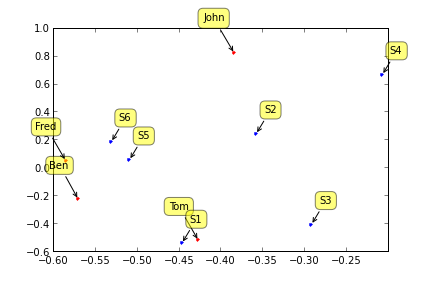
\includegraphics[height=6cm]{svdrecom_1.png}

Cok guzel! SVD bize urun bazinda sezon 5 ve 6'nin bir kume
olusturdugunu, Ben ve Fred'in de kisi bazinda ayri bir kume oldugunu
gosterdi.

Azaltilmis boyutlari nasil kullaniriz? Yeni bir kisiyi (mesela Bob)
ele alinca, bu kisinin verisini oncelikle aynen diger verilerin
indirgendigi gibi azaltilmis boyuta "indirgememiz" gerekiyor. Cunku
artik islem yaptigimiz boyut orasi. Peki bu indirgemeyi nasil yapariz?
SVD genel formulunu hatirlarsak,

$$ A = USV $$

Azaltilmis ortamda

$$ A = U_k S_k V_k $$

Diyelim ki gitmek istedigimiz nokta azaltilmis $U$, o zaman $U_k$'yi tek
basina birakalim,

$$ A V_k^{-1} = U_k S V_k V_k^{-1} $$

$U_k,V_k$ matrisleri ortonormal, o zaman $V_k^{-1}V_k = I$ olacak,
yani yokolacak

$$ A V_k^{-1} = U_k S  $$

Benzer sekilde

$$  A V_k^{-1} S^{-1} = U_k $$

Cok fazla ters alma islemi var, her iki tarafin devrigini alalim

$$ (S^{-1})^T (V_k^{-1})^T A^T = U_k^T $$

$V_k^{-1} = V_k^T$ o zaman ustteki formul devrigin devrigini almak
demektir, yani tekrar basa donmus oluyoruz, demek ki $V_k$ degismeden
kaliyor

$$ (S^{-1})^T V_k A^T = U_k^T $$

$S$ ise kosegen matris, onun tersi yine kosegen, kosegen matrisin devrigi
yine kendisi

$$ S^{-1} V_k A^T = U_k^T $$

Bazi kod ispatlari, $u$'nun ortonormal olmasi:

\begin{minted}[fontsize=\footnotesize]{python}
print np.dot(u.T,u)
\end{minted}

\begin{verbatim}
[[  1.00000000e+00   4.83147593e-18]
 [  4.83147593e-18   1.00000000e+00]]
\end{verbatim}

Dogal olarak ..e-17 gibi bir sayi sifira cok yakin, yani sifir kabul
edilebilir. Devrik ve tersin ayni oldugunu gosterelim: Iki matrisi
birbirinden cikartip, cok kucuk bir sayidan buyukluge gore filtreleme
yapalim, ve sonuc icinde bir tane bile True olup olmadigini kontrol
edelim,

\begin{minted}[fontsize=\footnotesize]{python}
print not any(U.T-la.inv(U) > 1e-15)
\end{minted}

\begin{verbatim}
True
\end{verbatim}

Yeni Bob verisi 

\begin{minted}[fontsize=\footnotesize]{python}
bob = np.array([5,5,0,0,0,5]) 
\end{minted}

O zaman 

\begin{minted}[fontsize=\footnotesize]{python}
print bob.T.shape
print u.shape
S_k = np.eye(2)*Sigma[:2]
bob_2d = np.dot(np.dot(la.inv(S_k),vt.T),bob.T)
print bob_2d
\end{minted}

\begin{verbatim}
(6,)
(4, 2)
[-0.37752201 -0.08020351]
\end{verbatim}

Ustte \verb!eye! ve \verb!Sigma! ile ufak bir takla attik, bunun sebebi
\verb!svd! cagrisindan gelen \verb!Sigma!  sonucunun bir vektor olmasi ama
ustteki islem icin kosegen bir "matrise" ihtiyacimiz olmasi. Eger birim
(identity) matrisini alip onu \verb!Sigma! ile carparsak, bu kosegen
matrisi elde ederiz.

Simdi mesela kosinus benzerligi kullanarak bu izdusumlenmis yeni
vektorun hangi diger vektorlere benzedigini bulalim.

\begin{minted}[fontsize=\footnotesize]{python}
for i,user in enumerate(u):
   print data.index[i],cos_sim(user,bob_2d)
\end{minted}

\begin{verbatim}
Ben 0.993397525045
Tom 0.891664622942
John 0.612561691287
Fred 0.977685793579
\end{verbatim}

Sonuca gore yeni kullanici Bob, en cok Ben ve Fred'e benziyor. Sonuca
eristik! Artik bu iki kullanicinin yuksek not verdigi ama Bob'un hic
not vermedigi sezonlari alip Bob'a tavsiye olarak sunabiliriz.

Movielens 1M Verisi

Bu veri seti 6000 kullanici tarafindan yaklasik 4000 tane filme
verilen not / derece (rating) verisini iceriyor, 1 milyon tane not
verilmis, yani 4000 * 6000 = 24 milyon olasilik icinde sadece 1 milyon
veri noktasi dolu. Bu oldukca seyrek bir matris demektir.

Verinin ham hali diger ders notlarimizi iceren ust dizinlerde var, veriyi
SVD ile kullanilir hale getirmek icin bu dizindeki \verb!movielens_prep.py!
adli script kullanilir. Islem bitince \verb!movielens.csv! adli bir dosya
script'te gorulen yere yazilacak. Bu dosyada olmayan derecelendirmeler,
verilmemis notlar bos olacaktir. Bu bosluklari sifirlarsak, seyrek matrisi
o noktalari atlar. Ardindan bu seyrek matris uzerinde seyrek SVD
isletilebilir. Bu normal SVD'den daha hizli isleyecektir.

Tavsiye kodlamamiz icin yazinin basinda anlatilan teknigi
kullanacagiz, film verisi uzerinde boyut azaltilmasi yapilacak, benzer
kullanici bulunacak, ve herhangi bir yeni kullanici / film
kombinasyonu icin bu diger benzer kullanicinin o filme verdigi not
baz alinacak. 

Veriyi egitim ve test olarak iki parcaya bolecegiz. SVD egitim bolumu
uzerinde isletilecek.

Bu baglamda, onemli bir diger konu eksik veri noktalarinin SVD
sonuclarini nasil etkileyecegi. Sonucta eksik yerler \verb!nan!,
oradan sifir yapilip ardindan seyrek matris kodlamasi uzerinden
"atlaniyor" olabilir, fakat bu degerler atlaniyor (yani hizli
isleniyor, depolaniyor) olsa bile, onlarin sifir olmasinin bir anlami
yok mudur? Evet vardir. Not bakimindan sifir da bir not'tur, ve bu
sebeple sonuclari istenmeyen bicimde etkileyebilir.

O zaman mevcut veriyi oyle bir degistirelim ki verilmemis notlar, yani
sifir degerleri sonucu fazla degistirmesin.

Bunu yapmanin yollarindan biri her film icin bir ortalama not degeri
hesaplamak, ve bu ortalama degeri o filme verilen tum not
degerlerinden cikartmaktir. Bu isleme "sifir cevresinde merkezlemek"
ismi de verilir, hakikaten mesela film j icin ortalama 3 ise, 5 degeri
2, 3 degeri sifir, 2 degeri -1 haline gelecektir. Bu bir ilerlemedir
cunku ortalama 3 degeri zaten bizim icin "onemsiz" bir degerdir,
tavsiye problemi baglaminda bizim en cok ilgilendigimiz sevilen
filmler, ve sevilmeyen filmler. Bu degerler sirasiyla arti ve eksi
degerlere donusecekler, ve SVD bu farkliligi matematiksel olarak
kullanabilme yetenegine sahip.

Altta Pandas \verb!mean! cagrisi ile bu islemin yapildigini
goruyoruz, dikkat, Pandas dataframe icinde \verb!nan! degerleri
olacaktir, ve Pandas bu degerleri atlamasi gerektigini bilir, yani bu
degerler ortalamaya etki etmez. Ardindan merkezleme islemi egitim
verisi uzerinde uygulaniyor.

\begin{minted}[fontsize=\footnotesize]{python}
import pandas as pd, os
import scipy.sparse as sps
df = pd.read_csv("%s/Downloads/movielens.csv" % os.environ['HOME'] ,sep=';')
print df.shape
df = df.ix[:,1:] # id kolonunu atla
df = df.ix[:,:3700] # sadece filmleri al
df_train = df.copy().ix[:5000,:]
df_test = df.copy().ix[5001:,:]
df_train[np.isnan(df_train)] = 0.0
movie_avg_rating = np.array(df_train.mean(axis=0))
df_train = df_train - movie_avg_rating
dfs_train = sps.coo_matrix(df_train)

df_train = np.array(df_train)
df_test = np.array(df_test)

print df_train.shape
print df_test.shape

__top_k__ = 10
import scipy.sparse.linalg as slin
import scipy.linalg as la
U,Sigma,V=slin.svds(dfs_train,k=__top_k__)
print U.shape, Sigma.shape, V.shape
Sigma = np.diag(Sigma)
\end{minted}

\begin{verbatim}
(6040, 3731)
(5001, 3700)
(1039, 3700)
(5001, 10) (10,) (10, 3700)
\end{verbatim}

Altta test verisi uzerinde satir satir ilerliyoruz, ve her satir (test
kullanicisi) icinde film film ilerliyoruz. "Verilmis bir not" ariyoruz
(cogunlukla not verilmemis oluyor cunku), ve buldugumuz zaman artik
elimizde test edebilecegimiz bir sey var, o notu "sifirlayip" vektorun
geri kalanini azaltilmis boyuta yansitiyoruz, ve sonra o boyuttaki tum
diger $U$ vektorleri icinde arama yapiyoruz, en yakin diger
kullaniciyi buluyoruz ve onun bu filme verdigi notu tahminimiz olarak
kullaniyoruz.

Altta eger bulunan diger kullanici o filme not vermemisse, basitlestirme
amacli olarak, o filmi atladik. Gercek dunya sartlarinda filme not vermis
ve yakin olan (en yakin olmasa da) ikinci, ucuncu kullanicilar bulunup
onlarin notu kullanilabilir. Hatta en yakin k tane kullanicinin ortalamasi
alinabilir (o kullanicilar kNN gibi bir metotla bulunur belki), vs.

\begin{minted}[fontsize=\footnotesize]{python}
def euclid(inA,inB):
    return 1.0/(1.0 + la.norm(inA - inB))
    
rmse = 0; n = 0
for i,test_row in enumerate(df_test):
    for j, test_val in enumerate(test_row):
        # nan olmayan bir not buluncaya kadar ara
        if np.isnan(test_val): continue	
        # bulduk, test satirini tamamen kopyala ve bulunan notu silerek
        # onu nan / sifir haline getir cunku yansitma (projection) oncesi
        # o notu 'bilmiyormus gibi' yapmamiz lazim. 
	curr = test_row.copy()
        curr[j] = np.nan
        curr[np.isnan(curr)] = 0.

	proj_row = np.dot(np.dot(la.inv(Sigma),V),curr)

	sims = np.array(map(lambda x: euclid(x, proj_row), U[:,:__top_k__]))
	isim = np.argmax(sims)

	# eger bulunan kullanici o filme not vermemisse atla
	if np.isnan(df.ix[isim, j]): continue

	# egitim verisinde notlar sifir etrafinda ortalanmis, tekrar
	# normal haline dondur
	est = df_train[isim, j]+movie_avg_rating[j]

	# gercek not
	real = df_test[i, j]

	print i, 'icin en yakin', isim, 'urun',j, 'icin oy', est, 'gercek', real
        rmse += (real-est)**2
        n += 1
	break # her kullanici icin tek film test et
    if i == 20: break # 20 kullanici test et

print "rmse", np.sqrt(rmse / n)
\end{minted}

\begin{verbatim}
0 icin en yakin 1903 urun 144 icin oy 5.0 gercek 5.0
1 icin en yakin 239 urun 144 icin oy 5.0 gercek 5.0
2 icin en yakin 2045 urun 844 icin oy 4.0 gercek 4.0
3 icin en yakin 4636 urun 0 icin oy 3.0 gercek 4.0
4 icin en yakin 139 urun 845 icin oy 4.0 gercek 5.0
5 icin en yakin 427 urun 1107 icin oy 4.0 gercek 5.0
6 icin en yakin 3620 urun 31 icin oy 4.0 gercek 4.0
7 icin en yakin 1870 urun 0 icin oy 4.0 gercek 3.0
8 icin en yakin 4816 urun 106 icin oy 5.0 gercek 5.0
9 icin en yakin 3511 urun 0 icin oy 3.0 gercek 4.0
10 icin en yakin 3973 urun 1212 icin oy 5.0 gercek 4.0
11 icin en yakin 2554 urun 287 icin oy 4.0 gercek 5.0
12 icin en yakin 4733 urun 31 icin oy 4.0 gercek 3.0
13 icin en yakin 2339 urun 9 icin oy 4.0 gercek 3.0
14 icin en yakin 3036 urun 10 icin oy 4.0 gercek 3.0
15 icin en yakin 2748 urun 253 icin oy 5.0 gercek 5.0
16 icin en yakin 450 urun 16 icin oy 4.0 gercek 4.0
17 icin en yakin 1133 urun 9 icin oy 5.0 gercek 2.0
18 icin en yakin 3037 urun 253 icin oy 5.0 gercek 4.0
19 icin en yakin 1266 urun 107 icin oy 3.0 gercek 3.0
20 icin en yakin 537 urun 253 icin oy 5.0 gercek 5.0
rmse 0.975900072949
\end{verbatim}

Sonuc fena degil. Tavsiye programlarinda RMSE 0.9 civari iyi olarak
bilinir, Netflix yarismasinda [3] mesela kazanan algoritma RMSE 0.85'e
erismistir.

Kaynaklar

[1] \url{http://www.igvita.com/2007/01/15/svd-recommendation-system-in-ruby/}

[2] Harrington, P., Machine Learning in Action

[3] \url{http://en.wikipedia.org/wiki/Netflix_Prize}

[4] \url{http://stats.stackexchange.com/questions/31096/how-do-i-use-the-svd-in-collaborative-filtering}

\end{document}
